
%(BEGIN_QUESTION)
% Copyright 2010, Tony R. Kuphaldt, released under the Creative Commons Attribution License (v 1.0)
% This means you may do almost anything with this work of mine, so long as you give me proper credit

Anta at du må måle temperaturen i en ovn med bare en 1000 $\Omega$ RTD ($\alpha$ = 0.00385), en 1.75 k$\Omega$ presisjonsmotstand og et batteri med ukjent spenning:

$$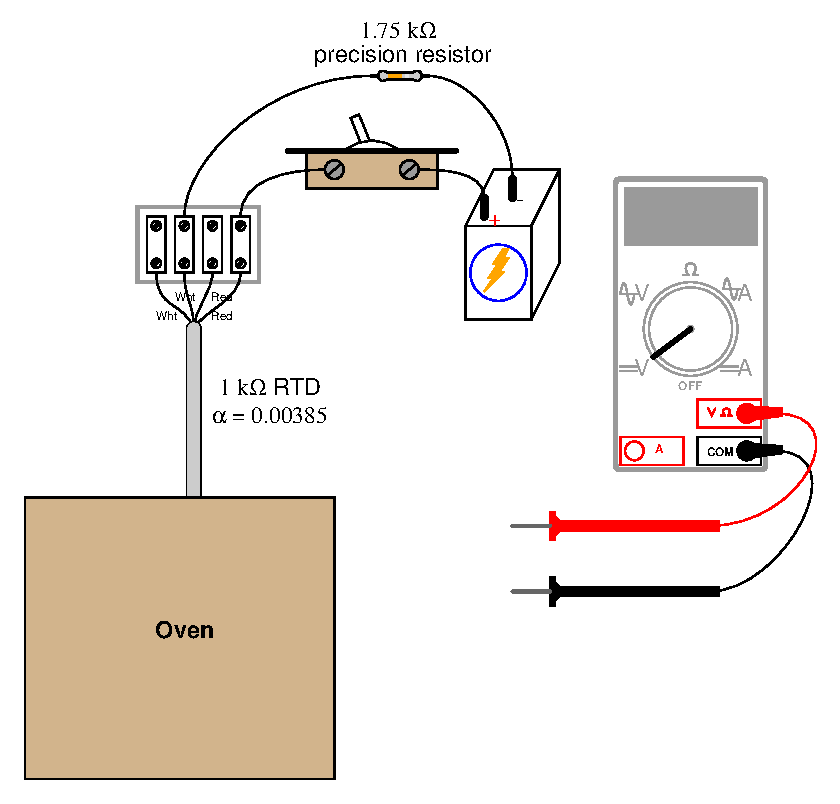
\includegraphics[width=15.5cm]{i00632x01.eps}$$

Når du slår på bryteren måler du 1.32 volt over motstanden og 1.22 volt over RTD-en. Beregn ovnstemperaturen ut fra disse målingene, og forklar også hvorfor det er viktig å ta disse målingene {\it raskt} etter at bryteren er slått på.

\underbar{file i00632no}
%(END_QUESTION)





%(BEGIN_ANSWER)

$R_{RTD}$ = 1.617 k$\Omega$

\vskip 10pt

$T_{oven}$ = 160.4 $^{o}$C = 320.7 $^{o}$F (beregnet fra formel, ikke fra tabell)

\vskip 10pt

Spenningsmålingene må tas svært raskt etter at bryteren er slått på for å unngå målefeil på grunn av "selvoppvarming" i RTD-en.

%(END_ANSWER)





%(BEGIN_NOTES)


%INDEX% Måling, temperatur: RTD

%(END_NOTES)
